\section{Application scenarios}
\label{sec:application_scenarios}

As was mentioned in \autoref{sec:motivation}, there are a number of ways to apply
our prediction methodology in a practical visualization system. 
To this end I show two application scenarios where my method can be
used to control the number of samples to maintain interactive 
rates.  I show how our method may be used 
to sample the simulation in order
to maintain a desired frame rate and to subsample an existing dataset in
order to attain interactive frame rates.

\subsection{Constrain sampling}
\label{sec:constrainsampling}

\begin{figure}[h]
\centering
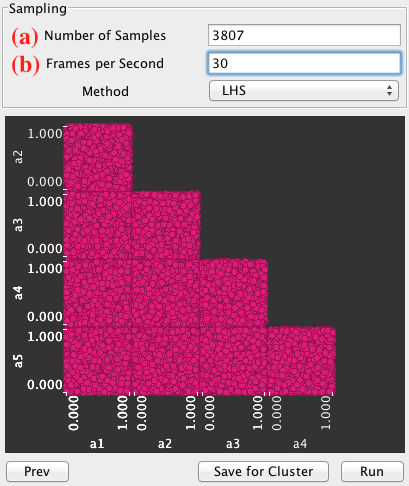
\includegraphics[width=7cm]{sampler_fps}
\caption[Using rendering time prediction to constrain sampling]{%
  A prototypical example use case for my prediction formula,
  \autoref{eq:calib-acttotal-H}. The user
  is able to either enter the number of sample points directly in field (a)
  and the system displays the expected fps in (b) or enter the desired fps
  in (b) first and the system calculates the number of sample points.
}
\label{fig:sampler}
\end{figure}


\autoref{fig:sampler} is a dialog box for the Tuner~\cite{Torsney-Weir:2011} system. 
The task is
to enter the number of sample points to take from the simulation. The dialog
is driven by \autoref{eq:calib-acttotal-H}. When the user changes the number of
samples directly (a), the dialog computes the expected frame rate and displays
that to the user in (b). As an alternative method, the user may value
interactivity highly and consequently selects the number of sample points to
take by entering the desired frame rate (b) and letting the system select the
number of samples.

\subsection{Subsample points}
\label{sec:subsamplepoints}

The goal of this algorithm, presented as \autoref{algo:subsample} is to reduce the
sample size, $N$, such that the rendering time reaches an acceptable 30fps.
Normally this is done by removing samples from the set.  An issue with simply
removing points and rebuilding the Gaussian process model is that the
bandwidth parameters, $\theta$ will change.

In \autoref{fig:30fps_time} I show the trade-off between the radius, $r$, and the
number of points, $N$, that can be drawn in 30fps.  When subsampling data I
expect that the radius around each sample point increases as the number of
sample points decreases.
The goal of \autoref{algo:subsample} is to 
lower the number of sample points until this line is reached.

\begin{algorithm}
  \caption[Subsampling data to achieve interactive rendering time]{%
    A proposed algorithm for subsampling data in order to achieve
    interactive rendering times using the Gaussian process model
    with the HyperSlice rendering technique.
  }
  \label{algo:subsample}
  \begin{algorithmic}
    \Require Calibrated prediction formula $E[t_\text{total}^\text{H}](N, d, r)$,
             calibrated GP model parameters $\vec{\theta}$

    \State $t_\text{pred} \gets E[t_\text{total}^\text{H}](N, d, r)$\;
    \While{$t_\text{pred} < 30\text{fps}$}
      \State $N_\text{30fps} \gets$ Numerically solve $E[t_\text{total}^\text{H}](N, d, r)$ for an $N$ that will give 30fps rendering times\;
      \State Uniformly remove $N - N_\text{30fps}$ sample points\;
      \State $r' \gets$ Rebuild the GP model, thereby recomputing $r$\;
      \State $t_\text{pred} \gets E[t_\text{total}^\text{H}](N_\text{30fps}, d, r')$\;
    \EndWhile
  \end{algorithmic}
\end{algorithm}

In this fashion one can have a progressive rendering setup using 2 GP models, 
a low-resolution model for fast rendering and a high-resolution one for
detail views.  The system could dynamically switch between these two when
interacting.

\begin{figure}[h]
  \centering
  % Created by tikzDevice version 0.7.0 on 2014-07-31 11:05:07
% !TEX encoding = UTF-8 Unicode
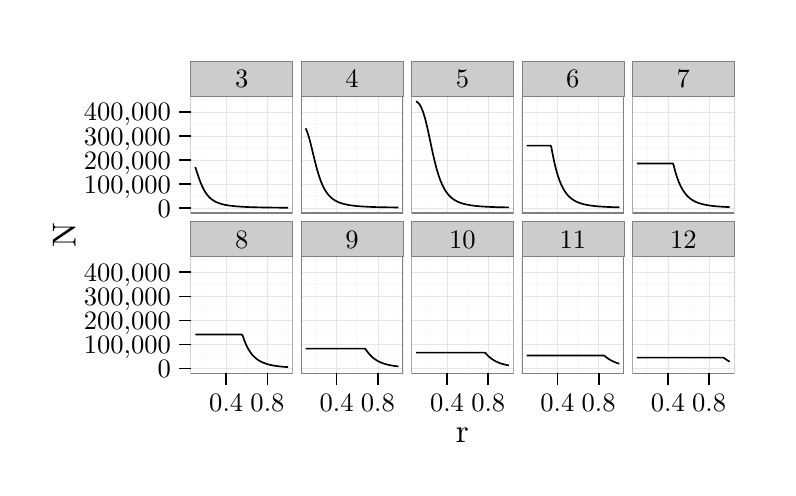
\begin{tikzpicture}[x=1pt,y=1pt]
\definecolor[named]{fillColor}{rgb}{1.00,1.00,1.00}
\path[use as bounding box,fill=fillColor,fill opacity=0.00] (0,0) rectangle (267.40,158.99);
\begin{scope}
\path[clip] (  0.00,  0.00) rectangle (267.40,158.99);
\definecolor[named]{drawColor}{rgb}{1.00,1.00,1.00}
\definecolor[named]{fillColor}{rgb}{1.00,1.00,1.00}

\path[draw=drawColor,line width= 0.6pt,line join=round,line cap=round,fill=fillColor] ( -0.00,  0.00) rectangle (267.40,158.99);
\end{scope}
\begin{scope}
\path[clip] ( 58.88, 92.00) rectangle ( 95.77,134.31);
\definecolor[named]{fillColor}{rgb}{1.00,1.00,1.00}

\path[fill=fillColor] ( 58.88, 92.00) rectangle ( 95.77,134.31);
\definecolor[named]{drawColor}{rgb}{0.98,0.98,0.98}

\path[draw=drawColor,line width= 0.6pt,line join=round] ( 58.88, 98.11) --
	( 95.77, 98.11);

\path[draw=drawColor,line width= 0.6pt,line join=round] ( 58.88,106.81) --
	( 95.77,106.81);

\path[draw=drawColor,line width= 0.6pt,line join=round] ( 58.88,115.52) --
	( 95.77,115.52);

\path[draw=drawColor,line width= 0.6pt,line join=round] ( 58.88,124.22) --
	( 95.77,124.22);

\path[draw=drawColor,line width= 0.6pt,line join=round] ( 58.88,132.92) --
	( 95.77,132.92);

\path[draw=drawColor,line width= 0.6pt,line join=round] ( 64.28, 92.00) --
	( 64.28,134.31);

\path[draw=drawColor,line width= 0.6pt,line join=round] ( 79.19, 92.00) --
	( 79.19,134.31);

\path[draw=drawColor,line width= 0.6pt,line join=round] ( 94.09, 92.00) --
	( 94.09,134.31);
\definecolor[named]{drawColor}{rgb}{0.90,0.90,0.90}

\path[draw=drawColor,line width= 0.2pt,line join=round] ( 58.88, 93.76) --
	( 95.77, 93.76);

\path[draw=drawColor,line width= 0.2pt,line join=round] ( 58.88,102.46) --
	( 95.77,102.46);

\path[draw=drawColor,line width= 0.2pt,line join=round] ( 58.88,111.16) --
	( 95.77,111.16);

\path[draw=drawColor,line width= 0.2pt,line join=round] ( 58.88,119.87) --
	( 95.77,119.87);

\path[draw=drawColor,line width= 0.2pt,line join=round] ( 58.88,128.57) --
	( 95.77,128.57);

\path[draw=drawColor,line width= 0.2pt,line join=round] ( 71.74, 92.00) --
	( 71.74,134.31);

\path[draw=drawColor,line width= 0.2pt,line join=round] ( 86.64, 92.00) --
	( 86.64,134.31);
\definecolor[named]{drawColor}{rgb}{0.00,0.00,0.00}

\path[draw=drawColor,line width= 0.6pt,line join=round] ( 60.56,108.63) --
	( 60.93,107.49) --
	( 61.30,106.35) --
	( 61.68,105.23) --
	( 62.05,104.17) --
	( 62.42,103.18) --
	( 62.79,102.27) --
	( 63.17,101.43) --
	( 63.54,100.68) --
	( 63.91,100.01) --
	( 64.28, 99.40) --
	( 64.66, 98.86) --
	( 65.03, 98.39) --
	( 65.40, 97.96) --
	( 65.77, 97.58) --
	( 66.15, 97.25) --
	( 66.52, 96.95) --
	( 66.89, 96.68) --
	( 67.27, 96.44) --
	( 67.64, 96.23) --
	( 68.01, 96.03) --
	( 68.38, 95.86) --
	( 68.76, 95.71) --
	( 69.13, 95.57) --
	( 69.50, 95.44) --
	( 69.87, 95.33) --
	( 70.25, 95.22) --
	( 70.62, 95.13) --
	( 70.99, 95.04) --
	( 71.36, 94.96) --
	( 71.74, 94.89) --
	( 72.11, 94.83) --
	( 72.48, 94.76) --
	( 72.85, 94.71) --
	( 73.23, 94.66) --
	( 73.60, 94.61) --
	( 73.97, 94.57) --
	( 74.34, 94.53) --
	( 74.72, 94.49) --
	( 75.09, 94.45) --
	( 75.46, 94.42) --
	( 75.83, 94.39) --
	( 76.21, 94.36) --
	( 76.58, 94.34) --
	( 76.95, 94.31) --
	( 77.32, 94.29) --
	( 77.70, 94.27) --
	( 78.07, 94.25) --
	( 78.44, 94.23) --
	( 78.82, 94.21) --
	( 79.19, 94.19) --
	( 79.56, 94.18) --
	( 79.93, 94.16) --
	( 80.31, 94.15) --
	( 80.68, 94.14) --
	( 81.05, 94.12) --
	( 81.42, 94.11) --
	( 81.80, 94.10) --
	( 82.17, 94.09) --
	( 82.54, 94.08) --
	( 82.91, 94.07) --
	( 83.29, 94.06) --
	( 83.66, 94.05) --
	( 84.03, 94.04) --
	( 84.40, 94.04) --
	( 84.78, 94.03) --
	( 85.15, 94.02) --
	( 85.52, 94.01) --
	( 85.89, 94.01) --
	( 86.27, 94.00) --
	( 86.64, 94.00) --
	( 87.01, 93.99) --
	( 87.38, 93.99) --
	( 87.76, 93.98) --
	( 88.13, 93.98) --
	( 88.50, 93.97) --
	( 88.87, 93.97) --
	( 89.25, 93.96) --
	( 89.62, 93.96) --
	( 89.99, 93.95) --
	( 90.37, 93.95) --
	( 90.74, 93.95) --
	( 91.11, 93.94) --
	( 91.48, 93.94) --
	( 91.86, 93.94) --
	( 92.23, 93.93) --
	( 92.60, 93.93) --
	( 92.97, 93.93) --
	( 93.35, 93.93) --
	( 93.72, 93.92) --
	( 94.09, 93.92);
\definecolor[named]{drawColor}{rgb}{0.50,0.50,0.50}

\path[draw=drawColor,line width= 0.6pt,line join=round,line cap=round] ( 58.88, 92.00) rectangle ( 95.77,134.31);
\end{scope}
\begin{scope}
\path[clip] ( 98.78, 92.00) rectangle (135.66,134.31);
\definecolor[named]{fillColor}{rgb}{1.00,1.00,1.00}

\path[fill=fillColor] ( 98.78, 92.00) rectangle (135.66,134.31);
\definecolor[named]{drawColor}{rgb}{0.98,0.98,0.98}

\path[draw=drawColor,line width= 0.6pt,line join=round] ( 98.78, 98.11) --
	(135.66, 98.11);

\path[draw=drawColor,line width= 0.6pt,line join=round] ( 98.78,106.81) --
	(135.66,106.81);

\path[draw=drawColor,line width= 0.6pt,line join=round] ( 98.78,115.52) --
	(135.66,115.52);

\path[draw=drawColor,line width= 0.6pt,line join=round] ( 98.78,124.22) --
	(135.66,124.22);

\path[draw=drawColor,line width= 0.6pt,line join=round] ( 98.78,132.92) --
	(135.66,132.92);

\path[draw=drawColor,line width= 0.6pt,line join=round] (104.18, 92.00) --
	(104.18,134.31);

\path[draw=drawColor,line width= 0.6pt,line join=round] (119.08, 92.00) --
	(119.08,134.31);

\path[draw=drawColor,line width= 0.6pt,line join=round] (133.99, 92.00) --
	(133.99,134.31);
\definecolor[named]{drawColor}{rgb}{0.90,0.90,0.90}

\path[draw=drawColor,line width= 0.2pt,line join=round] ( 98.78, 93.76) --
	(135.66, 93.76);

\path[draw=drawColor,line width= 0.2pt,line join=round] ( 98.78,102.46) --
	(135.66,102.46);

\path[draw=drawColor,line width= 0.2pt,line join=round] ( 98.78,111.16) --
	(135.66,111.16);

\path[draw=drawColor,line width= 0.2pt,line join=round] ( 98.78,119.87) --
	(135.66,119.87);

\path[draw=drawColor,line width= 0.2pt,line join=round] ( 98.78,128.57) --
	(135.66,128.57);

\path[draw=drawColor,line width= 0.2pt,line join=round] (111.63, 92.00) --
	(111.63,134.31);

\path[draw=drawColor,line width= 0.2pt,line join=round] (126.54, 92.00) --
	(126.54,134.31);
\definecolor[named]{drawColor}{rgb}{0.00,0.00,0.00}

\path[draw=drawColor,line width= 0.6pt,line join=round] (100.46,122.63) --
	(100.83,121.78) --
	(101.20,120.76) --
	(101.57,119.58) --
	(101.95,118.25) --
	(102.32,116.81) --
	(102.69,115.29) --
	(103.06,113.74) --
	(103.44,112.19) --
	(103.81,110.67) --
	(104.18,109.21) --
	(104.55,107.83) --
	(104.93,106.54) --
	(105.30,105.34) --
	(105.67,104.25) --
	(106.04,103.26) --
	(106.42,102.36) --
	(106.79,101.55) --
	(107.16,100.82) --
	(107.53,100.17) --
	(107.91, 99.59) --
	(108.28, 99.07) --
	(108.65, 98.60) --
	(109.02, 98.19) --
	(109.40, 97.81) --
	(109.77, 97.48) --
	(110.14, 97.18) --
	(110.51, 96.91) --
	(110.89, 96.67) --
	(111.26, 96.45) --
	(111.63, 96.25) --
	(112.01, 96.07) --
	(112.38, 95.91) --
	(112.75, 95.76) --
	(113.12, 95.63) --
	(113.50, 95.51) --
	(113.87, 95.39) --
	(114.24, 95.29) --
	(114.61, 95.20) --
	(114.99, 95.12) --
	(115.36, 95.04) --
	(115.73, 94.97) --
	(116.10, 94.90) --
	(116.48, 94.84) --
	(116.85, 94.78) --
	(117.22, 94.73) --
	(117.59, 94.68) --
	(117.97, 94.64) --
	(118.34, 94.60) --
	(118.71, 94.56) --
	(119.08, 94.52) --
	(119.46, 94.49) --
	(119.83, 94.46) --
	(120.20, 94.43) --
	(120.57, 94.40) --
	(120.95, 94.38) --
	(121.32, 94.35) --
	(121.69, 94.33) --
	(122.06, 94.31) --
	(122.44, 94.29) --
	(122.81, 94.27) --
	(123.18, 94.25) --
	(123.56, 94.24) --
	(123.93, 94.22) --
	(124.30, 94.21) --
	(124.67, 94.19) --
	(125.05, 94.18) --
	(125.42, 94.17) --
	(125.79, 94.16) --
	(126.16, 94.15) --
	(126.54, 94.14) --
	(126.91, 94.13) --
	(127.28, 94.12) --
	(127.65, 94.11) --
	(128.03, 94.10) --
	(128.40, 94.09) --
	(128.77, 94.09) --
	(129.14, 94.08) --
	(129.52, 94.07) --
	(129.89, 94.07) --
	(130.26, 94.06) --
	(130.63, 94.06) --
	(131.01, 94.05) --
	(131.38, 94.05) --
	(131.75, 94.04) --
	(132.12, 94.04) --
	(132.50, 94.03) --
	(132.87, 94.03) --
	(133.24, 94.03) --
	(133.61, 94.02) --
	(133.99, 94.02);
\definecolor[named]{drawColor}{rgb}{0.50,0.50,0.50}

\path[draw=drawColor,line width= 0.6pt,line join=round,line cap=round] ( 98.78, 92.00) rectangle (135.66,134.31);
\end{scope}
\begin{scope}
\path[clip] (138.68, 92.00) rectangle (175.56,134.31);
\definecolor[named]{fillColor}{rgb}{1.00,1.00,1.00}

\path[fill=fillColor] (138.68, 92.00) rectangle (175.56,134.31);
\definecolor[named]{drawColor}{rgb}{0.98,0.98,0.98}

\path[draw=drawColor,line width= 0.6pt,line join=round] (138.68, 98.11) --
	(175.56, 98.11);

\path[draw=drawColor,line width= 0.6pt,line join=round] (138.68,106.81) --
	(175.56,106.81);

\path[draw=drawColor,line width= 0.6pt,line join=round] (138.68,115.52) --
	(175.56,115.52);

\path[draw=drawColor,line width= 0.6pt,line join=round] (138.68,124.22) --
	(175.56,124.22);

\path[draw=drawColor,line width= 0.6pt,line join=round] (138.68,132.92) --
	(175.56,132.92);

\path[draw=drawColor,line width= 0.6pt,line join=round] (144.08, 92.00) --
	(144.08,134.31);

\path[draw=drawColor,line width= 0.6pt,line join=round] (158.98, 92.00) --
	(158.98,134.31);

\path[draw=drawColor,line width= 0.6pt,line join=round] (173.88, 92.00) --
	(173.88,134.31);
\definecolor[named]{drawColor}{rgb}{0.90,0.90,0.90}

\path[draw=drawColor,line width= 0.2pt,line join=round] (138.68, 93.76) --
	(175.56, 93.76);

\path[draw=drawColor,line width= 0.2pt,line join=round] (138.68,102.46) --
	(175.56,102.46);

\path[draw=drawColor,line width= 0.2pt,line join=round] (138.68,111.16) --
	(175.56,111.16);

\path[draw=drawColor,line width= 0.2pt,line join=round] (138.68,119.87) --
	(175.56,119.87);

\path[draw=drawColor,line width= 0.2pt,line join=round] (138.68,128.57) --
	(175.56,128.57);

\path[draw=drawColor,line width= 0.2pt,line join=round] (151.53, 92.00) --
	(151.53,134.31);

\path[draw=drawColor,line width= 0.2pt,line join=round] (166.43, 92.00) --
	(166.43,134.31);
\definecolor[named]{drawColor}{rgb}{0.00,0.00,0.00}

\path[draw=drawColor,line width= 0.6pt,line join=round] (140.35,132.39) --
	(140.72,132.16) --
	(141.10,131.84) --
	(141.47,131.41) --
	(141.84,130.85) --
	(142.21,130.15) --
	(142.59,129.29) --
	(142.96,128.27) --
	(143.33,127.08) --
	(143.71,125.74) --
	(144.08,124.26) --
	(144.45,122.66) --
	(144.82,120.97) --
	(145.20,119.23) --
	(145.57,117.46) --
	(145.94,115.70) --
	(146.31,113.98) --
	(146.69,112.33) --
	(147.06,110.75) --
	(147.43,109.27) --
	(147.80,107.89) --
	(148.18,106.61) --
	(148.55,105.44) --
	(148.92,104.37) --
	(149.29,103.39) --
	(149.67,102.51) --
	(150.04,101.72) --
	(150.41,101.00) --
	(150.78,100.35) --
	(151.16, 99.77) --
	(151.53, 99.25) --
	(151.90, 98.78) --
	(152.27, 98.36) --
	(152.65, 97.98) --
	(153.02, 97.64) --
	(153.39, 97.33) --
	(153.76, 97.05) --
	(154.14, 96.80) --
	(154.51, 96.57) --
	(154.88, 96.36) --
	(155.26, 96.17) --
	(155.63, 96.00) --
	(156.00, 95.85) --
	(156.37, 95.71) --
	(156.75, 95.58) --
	(157.12, 95.46) --
	(157.49, 95.35) --
	(157.86, 95.26) --
	(158.24, 95.17) --
	(158.61, 95.08) --
	(158.98, 95.01) --
	(159.35, 94.94) --
	(159.73, 94.87) --
	(160.10, 94.81) --
	(160.47, 94.75) --
	(160.84, 94.70) --
	(161.22, 94.66) --
	(161.59, 94.61) --
	(161.96, 94.57) --
	(162.33, 94.53) --
	(162.71, 94.50) --
	(163.08, 94.46) --
	(163.45, 94.43) --
	(163.82, 94.40) --
	(164.20, 94.38) --
	(164.57, 94.35) --
	(164.94, 94.33) --
	(165.31, 94.31) --
	(165.69, 94.29) --
	(166.06, 94.27) --
	(166.43, 94.25) --
	(166.81, 94.23) --
	(167.18, 94.21) --
	(167.55, 94.20) --
	(167.92, 94.18) --
	(168.30, 94.17) --
	(168.67, 94.16) --
	(169.04, 94.15) --
	(169.41, 94.14) --
	(169.79, 94.12) --
	(170.16, 94.11) --
	(170.53, 94.11) --
	(170.90, 94.10) --
	(171.28, 94.09) --
	(171.65, 94.08) --
	(172.02, 94.07) --
	(172.39, 94.07) --
	(172.77, 94.06) --
	(173.14, 94.05) --
	(173.51, 94.05) --
	(173.88, 94.04);
\definecolor[named]{drawColor}{rgb}{0.50,0.50,0.50}

\path[draw=drawColor,line width= 0.6pt,line join=round,line cap=round] (138.68, 92.00) rectangle (175.56,134.31);
\end{scope}
\begin{scope}
\path[clip] (178.57, 92.00) rectangle (215.46,134.31);
\definecolor[named]{fillColor}{rgb}{1.00,1.00,1.00}

\path[fill=fillColor] (178.57, 92.00) rectangle (215.46,134.31);
\definecolor[named]{drawColor}{rgb}{0.98,0.98,0.98}

\path[draw=drawColor,line width= 0.6pt,line join=round] (178.57, 98.11) --
	(215.46, 98.11);

\path[draw=drawColor,line width= 0.6pt,line join=round] (178.57,106.81) --
	(215.46,106.81);

\path[draw=drawColor,line width= 0.6pt,line join=round] (178.57,115.52) --
	(215.46,115.52);

\path[draw=drawColor,line width= 0.6pt,line join=round] (178.57,124.22) --
	(215.46,124.22);

\path[draw=drawColor,line width= 0.6pt,line join=round] (178.57,132.92) --
	(215.46,132.92);

\path[draw=drawColor,line width= 0.6pt,line join=round] (183.97, 92.00) --
	(183.97,134.31);

\path[draw=drawColor,line width= 0.6pt,line join=round] (198.88, 92.00) --
	(198.88,134.31);

\path[draw=drawColor,line width= 0.6pt,line join=round] (213.78, 92.00) --
	(213.78,134.31);
\definecolor[named]{drawColor}{rgb}{0.90,0.90,0.90}

\path[draw=drawColor,line width= 0.2pt,line join=round] (178.57, 93.76) --
	(215.46, 93.76);

\path[draw=drawColor,line width= 0.2pt,line join=round] (178.57,102.46) --
	(215.46,102.46);

\path[draw=drawColor,line width= 0.2pt,line join=round] (178.57,111.16) --
	(215.46,111.16);

\path[draw=drawColor,line width= 0.2pt,line join=round] (178.57,119.87) --
	(215.46,119.87);

\path[draw=drawColor,line width= 0.2pt,line join=round] (178.57,128.57) --
	(215.46,128.57);

\path[draw=drawColor,line width= 0.2pt,line join=round] (191.43, 92.00) --
	(191.43,134.31);

\path[draw=drawColor,line width= 0.2pt,line join=round] (206.33, 92.00) --
	(206.33,134.31);
\definecolor[named]{drawColor}{rgb}{0.00,0.00,0.00}

\path[draw=drawColor,line width= 0.6pt,line join=round] (180.25,116.38) --
	(180.62,116.38) --
	(180.99,116.38) --
	(181.37,116.38) --
	(181.74,116.38) --
	(182.11,116.38) --
	(182.48,116.38) --
	(182.86,116.38) --
	(183.23,116.38) --
	(183.60,116.38) --
	(183.97,116.38) --
	(184.35,116.38) --
	(184.72,116.38) --
	(185.09,116.38) --
	(185.46,116.38) --
	(185.84,116.38) --
	(186.21,116.38) --
	(186.58,116.38) --
	(186.95,116.38) --
	(187.33,116.38) --
	(187.70,116.38) --
	(188.07,116.38) --
	(188.45,116.38) --
	(188.82,116.38) --
	(189.19,116.01) --
	(189.56,113.97) --
	(189.94,112.08) --
	(190.31,110.34) --
	(190.68,108.76) --
	(191.05,107.32) --
	(191.43,106.02) --
	(191.80,104.85) --
	(192.17,103.79) --
	(192.54,102.85) --
	(192.92,102.00) --
	(193.29,101.23) --
	(193.66,100.55) --
	(194.03, 99.94) --
	(194.41, 99.39) --
	(194.78, 98.90) --
	(195.15, 98.46) --
	(195.52, 98.06) --
	(195.90, 97.71) --
	(196.27, 97.39) --
	(196.64, 97.10) --
	(197.01, 96.84) --
	(197.39, 96.60) --
	(197.76, 96.38) --
	(198.13, 96.19) --
	(198.50, 96.02) --
	(198.88, 95.86) --
	(199.25, 95.71) --
	(199.62, 95.58) --
	(200.00, 95.46) --
	(200.37, 95.35) --
	(200.74, 95.24) --
	(201.11, 95.15) --
	(201.49, 95.07) --
	(201.86, 94.99) --
	(202.23, 94.91) --
	(202.60, 94.85) --
	(202.98, 94.79) --
	(203.35, 94.73) --
	(203.72, 94.68) --
	(204.09, 94.63) --
	(204.47, 94.58) --
	(204.84, 94.54) --
	(205.21, 94.50) --
	(205.58, 94.47) --
	(205.96, 94.44) --
	(206.33, 94.40) --
	(206.70, 94.38) --
	(207.07, 94.35) --
	(207.45, 94.32) --
	(207.82, 94.30) --
	(208.19, 94.28) --
	(208.56, 94.26) --
	(208.94, 94.24) --
	(209.31, 94.22) --
	(209.68, 94.20) --
	(210.05, 94.19) --
	(210.43, 94.17) --
	(210.80, 94.16) --
	(211.17, 94.14) --
	(211.55, 94.13) --
	(211.92, 94.12) --
	(212.29, 94.11) --
	(212.66, 94.10) --
	(213.04, 94.09) --
	(213.41, 94.08) --
	(213.78, 94.07);
\definecolor[named]{drawColor}{rgb}{0.50,0.50,0.50}

\path[draw=drawColor,line width= 0.6pt,line join=round,line cap=round] (178.57, 92.00) rectangle (215.46,134.31);
\end{scope}
\begin{scope}
\path[clip] (218.47, 92.00) rectangle (255.35,134.31);
\definecolor[named]{fillColor}{rgb}{1.00,1.00,1.00}

\path[fill=fillColor] (218.47, 92.00) rectangle (255.35,134.31);
\definecolor[named]{drawColor}{rgb}{0.98,0.98,0.98}

\path[draw=drawColor,line width= 0.6pt,line join=round] (218.47, 98.11) --
	(255.35, 98.11);

\path[draw=drawColor,line width= 0.6pt,line join=round] (218.47,106.81) --
	(255.35,106.81);

\path[draw=drawColor,line width= 0.6pt,line join=round] (218.47,115.52) --
	(255.35,115.52);

\path[draw=drawColor,line width= 0.6pt,line join=round] (218.47,124.22) --
	(255.35,124.22);

\path[draw=drawColor,line width= 0.6pt,line join=round] (218.47,132.92) --
	(255.35,132.92);

\path[draw=drawColor,line width= 0.6pt,line join=round] (223.87, 92.00) --
	(223.87,134.31);

\path[draw=drawColor,line width= 0.6pt,line join=round] (238.77, 92.00) --
	(238.77,134.31);

\path[draw=drawColor,line width= 0.6pt,line join=round] (253.68, 92.00) --
	(253.68,134.31);
\definecolor[named]{drawColor}{rgb}{0.90,0.90,0.90}

\path[draw=drawColor,line width= 0.2pt,line join=round] (218.47, 93.76) --
	(255.35, 93.76);

\path[draw=drawColor,line width= 0.2pt,line join=round] (218.47,102.46) --
	(255.35,102.46);

\path[draw=drawColor,line width= 0.2pt,line join=round] (218.47,111.16) --
	(255.35,111.16);

\path[draw=drawColor,line width= 0.2pt,line join=round] (218.47,119.87) --
	(255.35,119.87);

\path[draw=drawColor,line width= 0.2pt,line join=round] (218.47,128.57) --
	(255.35,128.57);

\path[draw=drawColor,line width= 0.2pt,line join=round] (231.32, 92.00) --
	(231.32,134.31);

\path[draw=drawColor,line width= 0.2pt,line join=round] (246.23, 92.00) --
	(246.23,134.31);
\definecolor[named]{drawColor}{rgb}{0.00,0.00,0.00}

\path[draw=drawColor,line width= 0.6pt,line join=round] (220.15,109.90) --
	(220.52,109.90) --
	(220.89,109.90) --
	(221.26,109.90) --
	(221.64,109.90) --
	(222.01,109.90) --
	(222.38,109.90) --
	(222.75,109.90) --
	(223.13,109.90) --
	(223.50,109.90) --
	(223.87,109.90) --
	(224.24,109.90) --
	(224.62,109.90) --
	(224.99,109.90) --
	(225.36,109.90) --
	(225.73,109.90) --
	(226.11,109.90) --
	(226.48,109.90) --
	(226.85,109.90) --
	(227.22,109.90) --
	(227.60,109.90) --
	(227.97,109.90) --
	(228.34,109.90) --
	(228.71,109.90) --
	(229.09,109.90) --
	(229.46,109.90) --
	(229.83,109.90) --
	(230.20,109.90) --
	(230.58,109.90) --
	(230.95,109.90) --
	(231.32,109.90) --
	(231.70,109.90) --
	(232.07,109.90) --
	(232.44,109.90) --
	(232.81,109.90) --
	(233.19,109.90) --
	(233.56,108.72) --
	(233.93,107.31) --
	(234.30,106.03) --
	(234.68,104.88) --
	(235.05,103.84) --
	(235.42,102.91) --
	(235.79,102.07) --
	(236.17,101.31) --
	(236.54,100.64) --
	(236.91,100.03) --
	(237.28, 99.48) --
	(237.66, 98.99) --
	(238.03, 98.54) --
	(238.40, 98.14) --
	(238.77, 97.78) --
	(239.15, 97.46) --
	(239.52, 97.17) --
	(239.89, 96.90) --
	(240.26, 96.66) --
	(240.64, 96.44) --
	(241.01, 96.24) --
	(241.38, 96.06) --
	(241.75, 95.90) --
	(242.13, 95.75) --
	(242.50, 95.61) --
	(242.87, 95.49) --
	(243.25, 95.38) --
	(243.62, 95.27) --
	(243.99, 95.18) --
	(244.36, 95.09) --
	(244.74, 95.01) --
	(245.11, 94.93) --
	(245.48, 94.86) --
	(245.85, 94.80) --
	(246.23, 94.74) --
	(246.60, 94.69) --
	(246.97, 94.64) --
	(247.34, 94.59) --
	(247.72, 94.55) --
	(248.09, 94.51) --
	(248.46, 94.47) --
	(248.83, 94.44) --
	(249.21, 94.41) --
	(249.58, 94.38) --
	(249.95, 94.35) --
	(250.32, 94.32) --
	(250.70, 94.30) --
	(251.07, 94.28) --
	(251.44, 94.26) --
	(251.81, 94.24) --
	(252.19, 94.22) --
	(252.56, 94.20) --
	(252.93, 94.18) --
	(253.30, 94.17) --
	(253.68, 94.15);
\definecolor[named]{drawColor}{rgb}{0.50,0.50,0.50}

\path[draw=drawColor,line width= 0.6pt,line join=round,line cap=round] (218.47, 92.00) rectangle (255.35,134.31);
\end{scope}
\begin{scope}
\path[clip] ( 58.88, 34.03) rectangle ( 95.77, 76.35);
\definecolor[named]{fillColor}{rgb}{1.00,1.00,1.00}

\path[fill=fillColor] ( 58.88, 34.03) rectangle ( 95.77, 76.35);
\definecolor[named]{drawColor}{rgb}{0.98,0.98,0.98}

\path[draw=drawColor,line width= 0.6pt,line join=round] ( 58.88, 40.15) --
	( 95.77, 40.15);

\path[draw=drawColor,line width= 0.6pt,line join=round] ( 58.88, 48.85) --
	( 95.77, 48.85);

\path[draw=drawColor,line width= 0.6pt,line join=round] ( 58.88, 57.55) --
	( 95.77, 57.55);

\path[draw=drawColor,line width= 0.6pt,line join=round] ( 58.88, 66.26) --
	( 95.77, 66.26);

\path[draw=drawColor,line width= 0.6pt,line join=round] ( 58.88, 74.96) --
	( 95.77, 74.96);

\path[draw=drawColor,line width= 0.6pt,line join=round] ( 64.28, 34.03) --
	( 64.28, 76.35);

\path[draw=drawColor,line width= 0.6pt,line join=round] ( 79.19, 34.03) --
	( 79.19, 76.35);

\path[draw=drawColor,line width= 0.6pt,line join=round] ( 94.09, 34.03) --
	( 94.09, 76.35);
\definecolor[named]{drawColor}{rgb}{0.90,0.90,0.90}

\path[draw=drawColor,line width= 0.2pt,line join=round] ( 58.88, 35.79) --
	( 95.77, 35.79);

\path[draw=drawColor,line width= 0.2pt,line join=round] ( 58.88, 44.50) --
	( 95.77, 44.50);

\path[draw=drawColor,line width= 0.2pt,line join=round] ( 58.88, 53.20) --
	( 95.77, 53.20);

\path[draw=drawColor,line width= 0.2pt,line join=round] ( 58.88, 61.90) --
	( 95.77, 61.90);

\path[draw=drawColor,line width= 0.2pt,line join=round] ( 58.88, 70.61) --
	( 95.77, 70.61);

\path[draw=drawColor,line width= 0.2pt,line join=round] ( 71.74, 34.03) --
	( 71.74, 76.35);

\path[draw=drawColor,line width= 0.2pt,line join=round] ( 86.64, 34.03) --
	( 86.64, 76.35);
\definecolor[named]{drawColor}{rgb}{0.00,0.00,0.00}

\path[draw=drawColor,line width= 0.6pt,line join=round] ( 60.56, 48.13) --
	( 60.93, 48.13) --
	( 61.30, 48.13) --
	( 61.68, 48.13) --
	( 62.05, 48.13) --
	( 62.42, 48.13) --
	( 62.79, 48.13) --
	( 63.17, 48.13) --
	( 63.54, 48.13) --
	( 63.91, 48.13) --
	( 64.28, 48.13) --
	( 64.66, 48.13) --
	( 65.03, 48.13) --
	( 65.40, 48.13) --
	( 65.77, 48.13) --
	( 66.15, 48.13) --
	( 66.52, 48.13) --
	( 66.89, 48.13) --
	( 67.27, 48.13) --
	( 67.64, 48.13) --
	( 68.01, 48.13) --
	( 68.38, 48.13) --
	( 68.76, 48.13) --
	( 69.13, 48.13) --
	( 69.50, 48.13) --
	( 69.87, 48.13) --
	( 70.25, 48.13) --
	( 70.62, 48.13) --
	( 70.99, 48.13) --
	( 71.36, 48.13) --
	( 71.74, 48.13) --
	( 72.11, 48.13) --
	( 72.48, 48.13) --
	( 72.85, 48.13) --
	( 73.23, 48.13) --
	( 73.60, 48.13) --
	( 73.97, 48.13) --
	( 74.34, 48.13) --
	( 74.72, 48.13) --
	( 75.09, 48.13) --
	( 75.46, 48.13) --
	( 75.83, 48.13) --
	( 76.21, 48.13) --
	( 76.58, 48.13) --
	( 76.95, 48.13) --
	( 77.32, 48.13) --
	( 77.70, 47.69) --
	( 78.07, 46.59) --
	( 78.44, 45.60) --
	( 78.82, 44.70) --
	( 79.19, 43.90) --
	( 79.56, 43.17) --
	( 79.93, 42.52) --
	( 80.31, 41.94) --
	( 80.68, 41.41) --
	( 81.05, 40.93) --
	( 81.42, 40.50) --
	( 81.80, 40.12) --
	( 82.17, 39.76) --
	( 82.54, 39.45) --
	( 82.91, 39.16) --
	( 83.29, 38.90) --
	( 83.66, 38.67) --
	( 84.03, 38.45) --
	( 84.40, 38.26) --
	( 84.78, 38.08) --
	( 85.15, 37.92) --
	( 85.52, 37.77) --
	( 85.89, 37.64) --
	( 86.27, 37.51) --
	( 86.64, 37.40) --
	( 87.01, 37.30) --
	( 87.38, 37.20) --
	( 87.76, 37.12) --
	( 88.13, 37.04) --
	( 88.50, 36.96) --
	( 88.87, 36.89) --
	( 89.25, 36.83) --
	( 89.62, 36.77) --
	( 89.99, 36.72) --
	( 90.37, 36.67) --
	( 90.74, 36.62) --
	( 91.11, 36.58) --
	( 91.48, 36.54) --
	( 91.86, 36.50) --
	( 92.23, 36.47) --
	( 92.60, 36.44) --
	( 92.97, 36.41) --
	( 93.35, 36.38) --
	( 93.72, 36.35) --
	( 94.09, 36.33);
\definecolor[named]{drawColor}{rgb}{0.50,0.50,0.50}

\path[draw=drawColor,line width= 0.6pt,line join=round,line cap=round] ( 58.88, 34.03) rectangle ( 95.77, 76.35);
\end{scope}
\begin{scope}
\path[clip] ( 98.78, 34.03) rectangle (135.66, 76.35);
\definecolor[named]{fillColor}{rgb}{1.00,1.00,1.00}

\path[fill=fillColor] ( 98.78, 34.03) rectangle (135.66, 76.35);
\definecolor[named]{drawColor}{rgb}{0.98,0.98,0.98}

\path[draw=drawColor,line width= 0.6pt,line join=round] ( 98.78, 40.15) --
	(135.66, 40.15);

\path[draw=drawColor,line width= 0.6pt,line join=round] ( 98.78, 48.85) --
	(135.66, 48.85);

\path[draw=drawColor,line width= 0.6pt,line join=round] ( 98.78, 57.55) --
	(135.66, 57.55);

\path[draw=drawColor,line width= 0.6pt,line join=round] ( 98.78, 66.26) --
	(135.66, 66.26);

\path[draw=drawColor,line width= 0.6pt,line join=round] ( 98.78, 74.96) --
	(135.66, 74.96);

\path[draw=drawColor,line width= 0.6pt,line join=round] (104.18, 34.03) --
	(104.18, 76.35);

\path[draw=drawColor,line width= 0.6pt,line join=round] (119.08, 34.03) --
	(119.08, 76.35);

\path[draw=drawColor,line width= 0.6pt,line join=round] (133.99, 34.03) --
	(133.99, 76.35);
\definecolor[named]{drawColor}{rgb}{0.90,0.90,0.90}

\path[draw=drawColor,line width= 0.2pt,line join=round] ( 98.78, 35.79) --
	(135.66, 35.79);

\path[draw=drawColor,line width= 0.2pt,line join=round] ( 98.78, 44.50) --
	(135.66, 44.50);

\path[draw=drawColor,line width= 0.2pt,line join=round] ( 98.78, 53.20) --
	(135.66, 53.20);

\path[draw=drawColor,line width= 0.2pt,line join=round] ( 98.78, 61.90) --
	(135.66, 61.90);

\path[draw=drawColor,line width= 0.2pt,line join=round] ( 98.78, 70.61) --
	(135.66, 70.61);

\path[draw=drawColor,line width= 0.2pt,line join=round] (111.63, 34.03) --
	(111.63, 76.35);

\path[draw=drawColor,line width= 0.2pt,line join=round] (126.54, 34.03) --
	(126.54, 76.35);
\definecolor[named]{drawColor}{rgb}{0.00,0.00,0.00}

\path[draw=drawColor,line width= 0.6pt,line join=round] (100.46, 43.01) --
	(100.83, 43.01) --
	(101.20, 43.01) --
	(101.57, 43.01) --
	(101.95, 43.01) --
	(102.32, 43.01) --
	(102.69, 43.01) --
	(103.06, 43.01) --
	(103.44, 43.01) --
	(103.81, 43.01) --
	(104.18, 43.01) --
	(104.55, 43.01) --
	(104.93, 43.01) --
	(105.30, 43.01) --
	(105.67, 43.01) --
	(106.04, 43.01) --
	(106.42, 43.01) --
	(106.79, 43.01) --
	(107.16, 43.01) --
	(107.53, 43.01) --
	(107.91, 43.01) --
	(108.28, 43.01) --
	(108.65, 43.01) --
	(109.02, 43.01) --
	(109.40, 43.01) --
	(109.77, 43.01) --
	(110.14, 43.01) --
	(110.51, 43.01) --
	(110.89, 43.01) --
	(111.26, 43.01) --
	(111.63, 43.01) --
	(112.01, 43.01) --
	(112.38, 43.01) --
	(112.75, 43.01) --
	(113.12, 43.01) --
	(113.50, 43.01) --
	(113.87, 43.01) --
	(114.24, 43.01) --
	(114.61, 43.01) --
	(114.99, 43.01) --
	(115.36, 43.01) --
	(115.73, 43.01) --
	(116.10, 43.01) --
	(116.48, 43.01) --
	(116.85, 43.01) --
	(117.22, 43.01) --
	(117.59, 43.01) --
	(117.97, 43.01) --
	(118.34, 43.01) --
	(118.71, 43.01) --
	(119.08, 43.01) --
	(119.46, 43.01) --
	(119.83, 43.01) --
	(120.20, 43.01) --
	(120.57, 43.01) --
	(120.95, 43.01) --
	(121.32, 43.01) --
	(121.69, 43.01) --
	(122.06, 42.92) --
	(122.44, 42.35) --
	(122.81, 41.83) --
	(123.18, 41.35) --
	(123.56, 40.91) --
	(123.93, 40.52) --
	(124.30, 40.15) --
	(124.67, 39.82) --
	(125.05, 39.51) --
	(125.42, 39.23) --
	(125.79, 38.98) --
	(126.16, 38.75) --
	(126.54, 38.53) --
	(126.91, 38.34) --
	(127.28, 38.16) --
	(127.65, 38.00) --
	(128.03, 37.85) --
	(128.40, 37.71) --
	(128.77, 37.59) --
	(129.14, 37.47) --
	(129.52, 37.36) --
	(129.89, 37.27) --
	(130.26, 37.18) --
	(130.63, 37.09) --
	(131.01, 37.02) --
	(131.38, 36.94) --
	(131.75, 36.88) --
	(132.12, 36.82) --
	(132.50, 36.76) --
	(132.87, 36.71) --
	(133.24, 36.66) --
	(133.61, 36.62) --
	(133.99, 36.58);
\definecolor[named]{drawColor}{rgb}{0.50,0.50,0.50}

\path[draw=drawColor,line width= 0.6pt,line join=round,line cap=round] ( 98.78, 34.03) rectangle (135.66, 76.35);
\end{scope}
\begin{scope}
\path[clip] (138.68, 34.03) rectangle (175.56, 76.35);
\definecolor[named]{fillColor}{rgb}{1.00,1.00,1.00}

\path[fill=fillColor] (138.68, 34.03) rectangle (175.56, 76.35);
\definecolor[named]{drawColor}{rgb}{0.98,0.98,0.98}

\path[draw=drawColor,line width= 0.6pt,line join=round] (138.68, 40.15) --
	(175.56, 40.15);

\path[draw=drawColor,line width= 0.6pt,line join=round] (138.68, 48.85) --
	(175.56, 48.85);

\path[draw=drawColor,line width= 0.6pt,line join=round] (138.68, 57.55) --
	(175.56, 57.55);

\path[draw=drawColor,line width= 0.6pt,line join=round] (138.68, 66.26) --
	(175.56, 66.26);

\path[draw=drawColor,line width= 0.6pt,line join=round] (138.68, 74.96) --
	(175.56, 74.96);

\path[draw=drawColor,line width= 0.6pt,line join=round] (144.08, 34.03) --
	(144.08, 76.35);

\path[draw=drawColor,line width= 0.6pt,line join=round] (158.98, 34.03) --
	(158.98, 76.35);

\path[draw=drawColor,line width= 0.6pt,line join=round] (173.88, 34.03) --
	(173.88, 76.35);
\definecolor[named]{drawColor}{rgb}{0.90,0.90,0.90}

\path[draw=drawColor,line width= 0.2pt,line join=round] (138.68, 35.79) --
	(175.56, 35.79);

\path[draw=drawColor,line width= 0.2pt,line join=round] (138.68, 44.50) --
	(175.56, 44.50);

\path[draw=drawColor,line width= 0.2pt,line join=round] (138.68, 53.20) --
	(175.56, 53.20);

\path[draw=drawColor,line width= 0.2pt,line join=round] (138.68, 61.90) --
	(175.56, 61.90);

\path[draw=drawColor,line width= 0.2pt,line join=round] (138.68, 70.61) --
	(175.56, 70.61);

\path[draw=drawColor,line width= 0.2pt,line join=round] (151.53, 34.03) --
	(151.53, 76.35);

\path[draw=drawColor,line width= 0.2pt,line join=round] (166.43, 34.03) --
	(166.43, 76.35);
\definecolor[named]{drawColor}{rgb}{0.00,0.00,0.00}

\path[draw=drawColor,line width= 0.6pt,line join=round] (140.35, 41.57) --
	(140.72, 41.57) --
	(141.10, 41.57) --
	(141.47, 41.57) --
	(141.84, 41.57) --
	(142.21, 41.57) --
	(142.59, 41.57) --
	(142.96, 41.57) --
	(143.33, 41.57) --
	(143.71, 41.57) --
	(144.08, 41.57) --
	(144.45, 41.57) --
	(144.82, 41.57) --
	(145.20, 41.57) --
	(145.57, 41.57) --
	(145.94, 41.57) --
	(146.31, 41.57) --
	(146.69, 41.57) --
	(147.06, 41.57) --
	(147.43, 41.57) --
	(147.80, 41.57) --
	(148.18, 41.57) --
	(148.55, 41.57) --
	(148.92, 41.57) --
	(149.29, 41.57) --
	(149.67, 41.57) --
	(150.04, 41.57) --
	(150.41, 41.57) --
	(150.78, 41.57) --
	(151.16, 41.57) --
	(151.53, 41.57) --
	(151.90, 41.57) --
	(152.27, 41.57) --
	(152.65, 41.57) --
	(153.02, 41.57) --
	(153.39, 41.57) --
	(153.76, 41.57) --
	(154.14, 41.57) --
	(154.51, 41.57) --
	(154.88, 41.57) --
	(155.26, 41.57) --
	(155.63, 41.57) --
	(156.00, 41.57) --
	(156.37, 41.57) --
	(156.75, 41.57) --
	(157.12, 41.57) --
	(157.49, 41.57) --
	(157.86, 41.57) --
	(158.24, 41.57) --
	(158.61, 41.57) --
	(158.98, 41.57) --
	(159.35, 41.57) --
	(159.73, 41.57) --
	(160.10, 41.57) --
	(160.47, 41.57) --
	(160.84, 41.57) --
	(161.22, 41.57) --
	(161.59, 41.57) --
	(161.96, 41.57) --
	(162.33, 41.57) --
	(162.71, 41.57) --
	(163.08, 41.57) --
	(163.45, 41.57) --
	(163.82, 41.57) --
	(164.20, 41.57) --
	(164.57, 41.57) --
	(164.94, 41.57) --
	(165.31, 41.54) --
	(165.69, 41.11) --
	(166.06, 40.71) --
	(166.43, 40.34) --
	(166.81, 40.00) --
	(167.18, 39.69) --
	(167.55, 39.40) --
	(167.92, 39.14) --
	(168.30, 38.90) --
	(168.67, 38.68) --
	(169.04, 38.47) --
	(169.41, 38.29) --
	(169.79, 38.12) --
	(170.16, 37.96) --
	(170.53, 37.81) --
	(170.90, 37.68) --
	(171.28, 37.56) --
	(171.65, 37.45) --
	(172.02, 37.34) --
	(172.39, 37.25) --
	(172.77, 37.16) --
	(173.14, 37.08) --
	(173.51, 37.00) --
	(173.88, 36.93);
\definecolor[named]{drawColor}{rgb}{0.50,0.50,0.50}

\path[draw=drawColor,line width= 0.6pt,line join=round,line cap=round] (138.68, 34.03) rectangle (175.56, 76.35);
\end{scope}
\begin{scope}
\path[clip] (178.57, 34.03) rectangle (215.46, 76.35);
\definecolor[named]{fillColor}{rgb}{1.00,1.00,1.00}

\path[fill=fillColor] (178.57, 34.03) rectangle (215.46, 76.35);
\definecolor[named]{drawColor}{rgb}{0.98,0.98,0.98}

\path[draw=drawColor,line width= 0.6pt,line join=round] (178.57, 40.15) --
	(215.46, 40.15);

\path[draw=drawColor,line width= 0.6pt,line join=round] (178.57, 48.85) --
	(215.46, 48.85);

\path[draw=drawColor,line width= 0.6pt,line join=round] (178.57, 57.55) --
	(215.46, 57.55);

\path[draw=drawColor,line width= 0.6pt,line join=round] (178.57, 66.26) --
	(215.46, 66.26);

\path[draw=drawColor,line width= 0.6pt,line join=round] (178.57, 74.96) --
	(215.46, 74.96);

\path[draw=drawColor,line width= 0.6pt,line join=round] (183.97, 34.03) --
	(183.97, 76.35);

\path[draw=drawColor,line width= 0.6pt,line join=round] (198.88, 34.03) --
	(198.88, 76.35);

\path[draw=drawColor,line width= 0.6pt,line join=round] (213.78, 34.03) --
	(213.78, 76.35);
\definecolor[named]{drawColor}{rgb}{0.90,0.90,0.90}

\path[draw=drawColor,line width= 0.2pt,line join=round] (178.57, 35.79) --
	(215.46, 35.79);

\path[draw=drawColor,line width= 0.2pt,line join=round] (178.57, 44.50) --
	(215.46, 44.50);

\path[draw=drawColor,line width= 0.2pt,line join=round] (178.57, 53.20) --
	(215.46, 53.20);

\path[draw=drawColor,line width= 0.2pt,line join=round] (178.57, 61.90) --
	(215.46, 61.90);

\path[draw=drawColor,line width= 0.2pt,line join=round] (178.57, 70.61) --
	(215.46, 70.61);

\path[draw=drawColor,line width= 0.2pt,line join=round] (191.43, 34.03) --
	(191.43, 76.35);

\path[draw=drawColor,line width= 0.2pt,line join=round] (206.33, 34.03) --
	(206.33, 76.35);
\definecolor[named]{drawColor}{rgb}{0.00,0.00,0.00}

\path[draw=drawColor,line width= 0.6pt,line join=round] (180.25, 40.53) --
	(180.62, 40.53) --
	(180.99, 40.53) --
	(181.37, 40.53) --
	(181.74, 40.53) --
	(182.11, 40.53) --
	(182.48, 40.53) --
	(182.86, 40.53) --
	(183.23, 40.53) --
	(183.60, 40.53) --
	(183.97, 40.53) --
	(184.35, 40.53) --
	(184.72, 40.53) --
	(185.09, 40.53) --
	(185.46, 40.53) --
	(185.84, 40.53) --
	(186.21, 40.53) --
	(186.58, 40.53) --
	(186.95, 40.53) --
	(187.33, 40.53) --
	(187.70, 40.53) --
	(188.07, 40.53) --
	(188.45, 40.53) --
	(188.82, 40.53) --
	(189.19, 40.53) --
	(189.56, 40.53) --
	(189.94, 40.53) --
	(190.31, 40.53) --
	(190.68, 40.53) --
	(191.05, 40.53) --
	(191.43, 40.53) --
	(191.80, 40.53) --
	(192.17, 40.53) --
	(192.54, 40.53) --
	(192.92, 40.53) --
	(193.29, 40.53) --
	(193.66, 40.53) --
	(194.03, 40.53) --
	(194.41, 40.53) --
	(194.78, 40.53) --
	(195.15, 40.53) --
	(195.52, 40.53) --
	(195.90, 40.53) --
	(196.27, 40.53) --
	(196.64, 40.53) --
	(197.01, 40.53) --
	(197.39, 40.53) --
	(197.76, 40.53) --
	(198.13, 40.53) --
	(198.50, 40.53) --
	(198.88, 40.53) --
	(199.25, 40.53) --
	(199.62, 40.53) --
	(200.00, 40.53) --
	(200.37, 40.53) --
	(200.74, 40.53) --
	(201.11, 40.53) --
	(201.49, 40.53) --
	(201.86, 40.53) --
	(202.23, 40.53) --
	(202.60, 40.53) --
	(202.98, 40.53) --
	(203.35, 40.53) --
	(203.72, 40.53) --
	(204.09, 40.53) --
	(204.47, 40.53) --
	(204.84, 40.53) --
	(205.21, 40.53) --
	(205.58, 40.53) --
	(205.96, 40.53) --
	(206.33, 40.53) --
	(206.70, 40.53) --
	(207.07, 40.53) --
	(207.45, 40.53) --
	(207.82, 40.53) --
	(208.19, 40.53) --
	(208.56, 40.30) --
	(208.94, 40.00) --
	(209.31, 39.71) --
	(209.68, 39.45) --
	(210.05, 39.20) --
	(210.43, 38.98) --
	(210.80, 38.76) --
	(211.17, 38.57) --
	(211.55, 38.39) --
	(211.92, 38.22) --
	(212.29, 38.06) --
	(212.66, 37.92) --
	(213.04, 37.78) --
	(213.41, 37.66) --
	(213.78, 37.54);
\definecolor[named]{drawColor}{rgb}{0.50,0.50,0.50}

\path[draw=drawColor,line width= 0.6pt,line join=round,line cap=round] (178.57, 34.03) rectangle (215.46, 76.35);
\end{scope}
\begin{scope}
\path[clip] (218.47, 34.03) rectangle (255.35, 76.35);
\definecolor[named]{fillColor}{rgb}{1.00,1.00,1.00}

\path[fill=fillColor] (218.47, 34.03) rectangle (255.35, 76.35);
\definecolor[named]{drawColor}{rgb}{0.98,0.98,0.98}

\path[draw=drawColor,line width= 0.6pt,line join=round] (218.47, 40.15) --
	(255.35, 40.15);

\path[draw=drawColor,line width= 0.6pt,line join=round] (218.47, 48.85) --
	(255.35, 48.85);

\path[draw=drawColor,line width= 0.6pt,line join=round] (218.47, 57.55) --
	(255.35, 57.55);

\path[draw=drawColor,line width= 0.6pt,line join=round] (218.47, 66.26) --
	(255.35, 66.26);

\path[draw=drawColor,line width= 0.6pt,line join=round] (218.47, 74.96) --
	(255.35, 74.96);

\path[draw=drawColor,line width= 0.6pt,line join=round] (223.87, 34.03) --
	(223.87, 76.35);

\path[draw=drawColor,line width= 0.6pt,line join=round] (238.77, 34.03) --
	(238.77, 76.35);

\path[draw=drawColor,line width= 0.6pt,line join=round] (253.68, 34.03) --
	(253.68, 76.35);
\definecolor[named]{drawColor}{rgb}{0.90,0.90,0.90}

\path[draw=drawColor,line width= 0.2pt,line join=round] (218.47, 35.79) --
	(255.35, 35.79);

\path[draw=drawColor,line width= 0.2pt,line join=round] (218.47, 44.50) --
	(255.35, 44.50);

\path[draw=drawColor,line width= 0.2pt,line join=round] (218.47, 53.20) --
	(255.35, 53.20);

\path[draw=drawColor,line width= 0.2pt,line join=round] (218.47, 61.90) --
	(255.35, 61.90);

\path[draw=drawColor,line width= 0.2pt,line join=round] (218.47, 70.61) --
	(255.35, 70.61);

\path[draw=drawColor,line width= 0.2pt,line join=round] (231.32, 34.03) --
	(231.32, 76.35);

\path[draw=drawColor,line width= 0.2pt,line join=round] (246.23, 34.03) --
	(246.23, 76.35);
\definecolor[named]{drawColor}{rgb}{0.00,0.00,0.00}

\path[draw=drawColor,line width= 0.6pt,line join=round] (220.15, 39.75) --
	(220.52, 39.75) --
	(220.89, 39.75) --
	(221.26, 39.75) --
	(221.64, 39.75) --
	(222.01, 39.75) --
	(222.38, 39.75) --
	(222.75, 39.75) --
	(223.13, 39.75) --
	(223.50, 39.75) --
	(223.87, 39.75) --
	(224.24, 39.75) --
	(224.62, 39.75) --
	(224.99, 39.75) --
	(225.36, 39.75) --
	(225.73, 39.75) --
	(226.11, 39.75) --
	(226.48, 39.75) --
	(226.85, 39.75) --
	(227.22, 39.75) --
	(227.60, 39.75) --
	(227.97, 39.75) --
	(228.34, 39.75) --
	(228.71, 39.75) --
	(229.09, 39.75) --
	(229.46, 39.75) --
	(229.83, 39.75) --
	(230.20, 39.75) --
	(230.58, 39.75) --
	(230.95, 39.75) --
	(231.32, 39.75) --
	(231.70, 39.75) --
	(232.07, 39.75) --
	(232.44, 39.75) --
	(232.81, 39.75) --
	(233.19, 39.75) --
	(233.56, 39.75) --
	(233.93, 39.75) --
	(234.30, 39.75) --
	(234.68, 39.75) --
	(235.05, 39.75) --
	(235.42, 39.75) --
	(235.79, 39.75) --
	(236.17, 39.75) --
	(236.54, 39.75) --
	(236.91, 39.75) --
	(237.28, 39.75) --
	(237.66, 39.75) --
	(238.03, 39.75) --
	(238.40, 39.75) --
	(238.77, 39.75) --
	(239.15, 39.75) --
	(239.52, 39.75) --
	(239.89, 39.75) --
	(240.26, 39.75) --
	(240.64, 39.75) --
	(241.01, 39.75) --
	(241.38, 39.75) --
	(241.75, 39.75) --
	(242.13, 39.75) --
	(242.50, 39.75) --
	(242.87, 39.75) --
	(243.25, 39.75) --
	(243.62, 39.75) --
	(243.99, 39.75) --
	(244.36, 39.75) --
	(244.74, 39.75) --
	(245.11, 39.75) --
	(245.48, 39.75) --
	(245.85, 39.75) --
	(246.23, 39.75) --
	(246.60, 39.75) --
	(246.97, 39.75) --
	(247.34, 39.75) --
	(247.72, 39.75) --
	(248.09, 39.75) --
	(248.46, 39.75) --
	(248.83, 39.75) --
	(249.21, 39.75) --
	(249.58, 39.75) --
	(249.95, 39.75) --
	(250.32, 39.75) --
	(250.70, 39.75) --
	(251.07, 39.75) --
	(251.44, 39.75) --
	(251.81, 39.51) --
	(252.19, 39.22) --
	(252.56, 38.96) --
	(252.93, 38.72) --
	(253.30, 38.51) --
	(253.68, 38.31);
\definecolor[named]{drawColor}{rgb}{0.50,0.50,0.50}

\path[draw=drawColor,line width= 0.6pt,line join=round,line cap=round] (218.47, 34.03) rectangle (255.35, 76.35);
\end{scope}
\begin{scope}
\path[clip] (  0.00,  0.00) rectangle (267.40,158.99);
\definecolor[named]{drawColor}{rgb}{0.50,0.50,0.50}
\definecolor[named]{fillColor}{rgb}{0.80,0.80,0.80}

\path[draw=drawColor,line width= 0.2pt,line join=round,line cap=round,fill=fillColor] ( 58.88,134.31) rectangle ( 95.77,146.95);
\definecolor[named]{drawColor}{rgb}{0.00,0.00,0.00}

\node[text=drawColor,anchor=base,inner sep=0pt, outer sep=0pt, scale=  0.96] at ( 77.32,137.33) { 3};
\end{scope}
\begin{scope}
\path[clip] (  0.00,  0.00) rectangle (267.40,158.99);
\definecolor[named]{drawColor}{rgb}{0.50,0.50,0.50}
\definecolor[named]{fillColor}{rgb}{0.80,0.80,0.80}

\path[draw=drawColor,line width= 0.2pt,line join=round,line cap=round,fill=fillColor] ( 98.78,134.31) rectangle (135.66,146.95);
\definecolor[named]{drawColor}{rgb}{0.00,0.00,0.00}

\node[text=drawColor,anchor=base,inner sep=0pt, outer sep=0pt, scale=  0.96] at (117.22,137.33) { 4};
\end{scope}
\begin{scope}
\path[clip] (  0.00,  0.00) rectangle (267.40,158.99);
\definecolor[named]{drawColor}{rgb}{0.50,0.50,0.50}
\definecolor[named]{fillColor}{rgb}{0.80,0.80,0.80}

\path[draw=drawColor,line width= 0.2pt,line join=round,line cap=round,fill=fillColor] (138.68,134.31) rectangle (175.56,146.95);
\definecolor[named]{drawColor}{rgb}{0.00,0.00,0.00}

\node[text=drawColor,anchor=base,inner sep=0pt, outer sep=0pt, scale=  0.96] at (157.12,137.33) { 5};
\end{scope}
\begin{scope}
\path[clip] (  0.00,  0.00) rectangle (267.40,158.99);
\definecolor[named]{drawColor}{rgb}{0.50,0.50,0.50}
\definecolor[named]{fillColor}{rgb}{0.80,0.80,0.80}

\path[draw=drawColor,line width= 0.2pt,line join=round,line cap=round,fill=fillColor] (178.57,134.31) rectangle (215.46,146.95);
\definecolor[named]{drawColor}{rgb}{0.00,0.00,0.00}

\node[text=drawColor,anchor=base,inner sep=0pt, outer sep=0pt, scale=  0.96] at (197.01,137.33) { 6};
\end{scope}
\begin{scope}
\path[clip] (  0.00,  0.00) rectangle (267.40,158.99);
\definecolor[named]{drawColor}{rgb}{0.50,0.50,0.50}
\definecolor[named]{fillColor}{rgb}{0.80,0.80,0.80}

\path[draw=drawColor,line width= 0.2pt,line join=round,line cap=round,fill=fillColor] (218.47,134.31) rectangle (255.35,146.95);
\definecolor[named]{drawColor}{rgb}{0.00,0.00,0.00}

\node[text=drawColor,anchor=base,inner sep=0pt, outer sep=0pt, scale=  0.96] at (236.91,137.33) { 7};
\end{scope}
\begin{scope}
\path[clip] (  0.00,  0.00) rectangle (267.40,158.99);
\definecolor[named]{drawColor}{rgb}{0.50,0.50,0.50}
\definecolor[named]{fillColor}{rgb}{0.80,0.80,0.80}

\path[draw=drawColor,line width= 0.2pt,line join=round,line cap=round,fill=fillColor] ( 58.88, 76.35) rectangle ( 95.77, 88.99);
\definecolor[named]{drawColor}{rgb}{0.00,0.00,0.00}

\node[text=drawColor,anchor=base,inner sep=0pt, outer sep=0pt, scale=  0.96] at ( 77.32, 79.36) { 8};
\end{scope}
\begin{scope}
\path[clip] (  0.00,  0.00) rectangle (267.40,158.99);
\definecolor[named]{drawColor}{rgb}{0.50,0.50,0.50}
\definecolor[named]{fillColor}{rgb}{0.80,0.80,0.80}

\path[draw=drawColor,line width= 0.2pt,line join=round,line cap=round,fill=fillColor] ( 98.78, 76.35) rectangle (135.66, 88.99);
\definecolor[named]{drawColor}{rgb}{0.00,0.00,0.00}

\node[text=drawColor,anchor=base,inner sep=0pt, outer sep=0pt, scale=  0.96] at (117.22, 79.36) { 9};
\end{scope}
\begin{scope}
\path[clip] (  0.00,  0.00) rectangle (267.40,158.99);
\definecolor[named]{drawColor}{rgb}{0.50,0.50,0.50}
\definecolor[named]{fillColor}{rgb}{0.80,0.80,0.80}

\path[draw=drawColor,line width= 0.2pt,line join=round,line cap=round,fill=fillColor] (138.68, 76.35) rectangle (175.56, 88.99);
\definecolor[named]{drawColor}{rgb}{0.00,0.00,0.00}

\node[text=drawColor,anchor=base,inner sep=0pt, outer sep=0pt, scale=  0.96] at (157.12, 79.36) {10};
\end{scope}
\begin{scope}
\path[clip] (  0.00,  0.00) rectangle (267.40,158.99);
\definecolor[named]{drawColor}{rgb}{0.50,0.50,0.50}
\definecolor[named]{fillColor}{rgb}{0.80,0.80,0.80}

\path[draw=drawColor,line width= 0.2pt,line join=round,line cap=round,fill=fillColor] (178.57, 76.35) rectangle (215.46, 88.99);
\definecolor[named]{drawColor}{rgb}{0.00,0.00,0.00}

\node[text=drawColor,anchor=base,inner sep=0pt, outer sep=0pt, scale=  0.96] at (197.01, 79.36) {11};
\end{scope}
\begin{scope}
\path[clip] (  0.00,  0.00) rectangle (267.40,158.99);
\definecolor[named]{drawColor}{rgb}{0.50,0.50,0.50}
\definecolor[named]{fillColor}{rgb}{0.80,0.80,0.80}

\path[draw=drawColor,line width= 0.2pt,line join=round,line cap=round,fill=fillColor] (218.47, 76.35) rectangle (255.35, 88.99);
\definecolor[named]{drawColor}{rgb}{0.00,0.00,0.00}

\node[text=drawColor,anchor=base,inner sep=0pt, outer sep=0pt, scale=  0.96] at (236.91, 79.36) {12};
\end{scope}
\begin{scope}
\path[clip] (  0.00,  0.00) rectangle (267.40,158.99);
\definecolor[named]{drawColor}{rgb}{0.00,0.00,0.00}

\node[text=drawColor,anchor=base east,inner sep=0pt, outer sep=0pt, scale=  0.96] at ( 51.77, 90.45) {0};

\node[text=drawColor,anchor=base east,inner sep=0pt, outer sep=0pt, scale=  0.96] at ( 51.77, 99.15) {100,000};

\node[text=drawColor,anchor=base east,inner sep=0pt, outer sep=0pt, scale=  0.96] at ( 51.77,107.86) {200,000};

\node[text=drawColor,anchor=base east,inner sep=0pt, outer sep=0pt, scale=  0.96] at ( 51.77,116.56) {300,000};

\node[text=drawColor,anchor=base east,inner sep=0pt, outer sep=0pt, scale=  0.96] at ( 51.77,125.27) {400,000};
\end{scope}
\begin{scope}
\path[clip] (  0.00,  0.00) rectangle (267.40,158.99);
\definecolor[named]{drawColor}{rgb}{0.00,0.00,0.00}

\path[draw=drawColor,line width= 0.6pt,line join=round] ( 54.61, 93.76) --
	( 58.88, 93.76);

\path[draw=drawColor,line width= 0.6pt,line join=round] ( 54.61,102.46) --
	( 58.88,102.46);

\path[draw=drawColor,line width= 0.6pt,line join=round] ( 54.61,111.16) --
	( 58.88,111.16);

\path[draw=drawColor,line width= 0.6pt,line join=round] ( 54.61,119.87) --
	( 58.88,119.87);

\path[draw=drawColor,line width= 0.6pt,line join=round] ( 54.61,128.57) --
	( 58.88,128.57);
\end{scope}
\begin{scope}
\path[clip] (  0.00,  0.00) rectangle (267.40,158.99);
\definecolor[named]{drawColor}{rgb}{0.00,0.00,0.00}

\node[text=drawColor,anchor=base east,inner sep=0pt, outer sep=0pt, scale=  0.96] at ( 51.77, 32.49) {0};

\node[text=drawColor,anchor=base east,inner sep=0pt, outer sep=0pt, scale=  0.96] at ( 51.77, 41.19) {100,000};

\node[text=drawColor,anchor=base east,inner sep=0pt, outer sep=0pt, scale=  0.96] at ( 51.77, 49.90) {200,000};

\node[text=drawColor,anchor=base east,inner sep=0pt, outer sep=0pt, scale=  0.96] at ( 51.77, 58.60) {300,000};

\node[text=drawColor,anchor=base east,inner sep=0pt, outer sep=0pt, scale=  0.96] at ( 51.77, 67.30) {400,000};
\end{scope}
\begin{scope}
\path[clip] (  0.00,  0.00) rectangle (267.40,158.99);
\definecolor[named]{drawColor}{rgb}{0.00,0.00,0.00}

\path[draw=drawColor,line width= 0.6pt,line join=round] ( 54.61, 35.79) --
	( 58.88, 35.79);

\path[draw=drawColor,line width= 0.6pt,line join=round] ( 54.61, 44.50) --
	( 58.88, 44.50);

\path[draw=drawColor,line width= 0.6pt,line join=round] ( 54.61, 53.20) --
	( 58.88, 53.20);

\path[draw=drawColor,line width= 0.6pt,line join=round] ( 54.61, 61.90) --
	( 58.88, 61.90);

\path[draw=drawColor,line width= 0.6pt,line join=round] ( 54.61, 70.61) --
	( 58.88, 70.61);
\end{scope}
\begin{scope}
\path[clip] (  0.00,  0.00) rectangle (267.40,158.99);
\definecolor[named]{drawColor}{rgb}{0.00,0.00,0.00}

\path[draw=drawColor,line width= 0.6pt,line join=round] ( 71.74, 29.77) --
	( 71.74, 34.03);

\path[draw=drawColor,line width= 0.6pt,line join=round] ( 86.64, 29.77) --
	( 86.64, 34.03);
\end{scope}
\begin{scope}
\path[clip] (  0.00,  0.00) rectangle (267.40,158.99);
\definecolor[named]{drawColor}{rgb}{0.00,0.00,0.00}

\node[text=drawColor,anchor=base,inner sep=0pt, outer sep=0pt, scale=  0.96] at ( 71.74, 20.31) {0.4};

\node[text=drawColor,anchor=base,inner sep=0pt, outer sep=0pt, scale=  0.96] at ( 86.64, 20.31) {0.8};
\end{scope}
\begin{scope}
\path[clip] (  0.00,  0.00) rectangle (267.40,158.99);
\definecolor[named]{drawColor}{rgb}{0.00,0.00,0.00}

\path[draw=drawColor,line width= 0.6pt,line join=round] (111.63, 29.77) --
	(111.63, 34.03);

\path[draw=drawColor,line width= 0.6pt,line join=round] (126.54, 29.77) --
	(126.54, 34.03);
\end{scope}
\begin{scope}
\path[clip] (  0.00,  0.00) rectangle (267.40,158.99);
\definecolor[named]{drawColor}{rgb}{0.00,0.00,0.00}

\node[text=drawColor,anchor=base,inner sep=0pt, outer sep=0pt, scale=  0.96] at (111.63, 20.31) {0.4};

\node[text=drawColor,anchor=base,inner sep=0pt, outer sep=0pt, scale=  0.96] at (126.54, 20.31) {0.8};
\end{scope}
\begin{scope}
\path[clip] (  0.00,  0.00) rectangle (267.40,158.99);
\definecolor[named]{drawColor}{rgb}{0.00,0.00,0.00}

\path[draw=drawColor,line width= 0.6pt,line join=round] (151.53, 29.77) --
	(151.53, 34.03);

\path[draw=drawColor,line width= 0.6pt,line join=round] (166.43, 29.77) --
	(166.43, 34.03);
\end{scope}
\begin{scope}
\path[clip] (  0.00,  0.00) rectangle (267.40,158.99);
\definecolor[named]{drawColor}{rgb}{0.00,0.00,0.00}

\node[text=drawColor,anchor=base,inner sep=0pt, outer sep=0pt, scale=  0.96] at (151.53, 20.31) {0.4};

\node[text=drawColor,anchor=base,inner sep=0pt, outer sep=0pt, scale=  0.96] at (166.43, 20.31) {0.8};
\end{scope}
\begin{scope}
\path[clip] (  0.00,  0.00) rectangle (267.40,158.99);
\definecolor[named]{drawColor}{rgb}{0.00,0.00,0.00}

\path[draw=drawColor,line width= 0.6pt,line join=round] (191.43, 29.77) --
	(191.43, 34.03);

\path[draw=drawColor,line width= 0.6pt,line join=round] (206.33, 29.77) --
	(206.33, 34.03);
\end{scope}
\begin{scope}
\path[clip] (  0.00,  0.00) rectangle (267.40,158.99);
\definecolor[named]{drawColor}{rgb}{0.00,0.00,0.00}

\node[text=drawColor,anchor=base,inner sep=0pt, outer sep=0pt, scale=  0.96] at (191.43, 20.31) {0.4};

\node[text=drawColor,anchor=base,inner sep=0pt, outer sep=0pt, scale=  0.96] at (206.33, 20.31) {0.8};
\end{scope}
\begin{scope}
\path[clip] (  0.00,  0.00) rectangle (267.40,158.99);
\definecolor[named]{drawColor}{rgb}{0.00,0.00,0.00}

\path[draw=drawColor,line width= 0.6pt,line join=round] (231.32, 29.77) --
	(231.32, 34.03);

\path[draw=drawColor,line width= 0.6pt,line join=round] (246.23, 29.77) --
	(246.23, 34.03);
\end{scope}
\begin{scope}
\path[clip] (  0.00,  0.00) rectangle (267.40,158.99);
\definecolor[named]{drawColor}{rgb}{0.00,0.00,0.00}

\node[text=drawColor,anchor=base,inner sep=0pt, outer sep=0pt, scale=  0.96] at (231.32, 20.31) {0.4};

\node[text=drawColor,anchor=base,inner sep=0pt, outer sep=0pt, scale=  0.96] at (246.23, 20.31) {0.8};
\end{scope}
\begin{scope}
\path[clip] (  0.00,  0.00) rectangle (267.40,158.99);
\definecolor[named]{drawColor}{rgb}{0.00,0.00,0.00}

\node[text=drawColor,anchor=base,inner sep=0pt, outer sep=0pt, scale=  1.20] at (157.12,  9.03) {r};
\end{scope}
\begin{scope}
\path[clip] (  0.00,  0.00) rectangle (267.40,158.99);
\definecolor[named]{drawColor}{rgb}{0.00,0.00,0.00}

\node[text=drawColor,rotate= 90.00,anchor=base,inner sep=0pt, outer sep=0pt, scale=  1.20] at ( 17.30, 84.17) {N};
\end{scope}
\end{tikzpicture}

  %\includegraphics[width=9cm]{30fps_time}
  \caption[Interactive rendering times for various dimensions]{%
    Average number of points that can be rendered in 30 frames per 
    second for the HyperSlice technique.
  }
  \label{fig:30fps_time}
\end{figure}

